\subsubsection{2.6. Mạng Kolgomorov-Arnold (KAN)}
\indent\indent Trong nhiều thập kỷ, kiến trúc MLP đã đóng vai trò là xương sống của hầu hết các mô hình học sâu. Tuy nhiên, MLP tồn tại những hạn chế trong khả năng biểu diễn phi tuyến đối với các đặc trưng phức tạp. Gần đây, Liu và cộng sự \cite{liu2025kankolmogorovarnoldnetworks} đã đề xuất một kiến trúc mới, gọi là mạng Kolmogorov-Arnold (KAN), kiến trúc này dựa trên định lý biểu diễn Kolmogorov-Arnold.\vspace{0.3cm}

\begin{figure}[H]
    \centering
    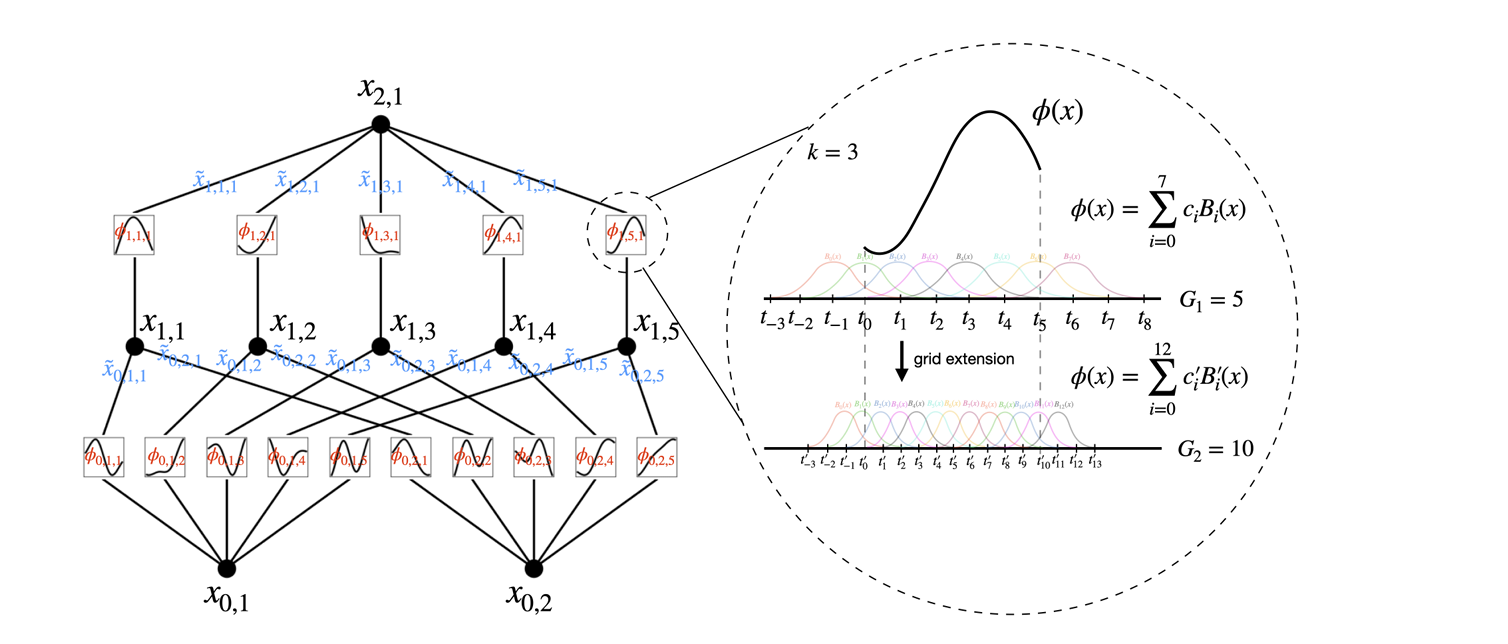
\includegraphics[width=0.8\linewidth]{images/part-02/chap-01/KAN.png}
    \vspace{0.5cm}
    \caption{Minh hoạ kiến trúc cơ bản của KAN}
    \label{fig:KAN}
\end{figure}

Khác với MLP -- nơi các hàm kích hoạt (activation functions) là cố định tại các nút và trọng số là các tham số học được trên các cạnh, KAN đảo ngược tư duy này: KAN không có trọng số tuyến tính, thay vào đó, mỗi cạnh kết nối chứa một hàm kích hoạt phi tuyến có thể học được (thường được tham số hóa bởi B-splines).\vspace{0.3cm}

Về mặt toán học, nếu MLP xấp xỉ hàm số thông qua tổ hợp tuyến tính và phi tuyến xen kẽ, thì một tầng KAN biểu diễn hàm mục tiêu $\Phi$ dựa trên công thức:
\[
    \Phi(\mathbf{x}) = \sum_{q=1}^{2n+1} \Phi_q \left( \sum_{p=1}^n \phi_{q,p}(x_p) \right)
\]
\indent Trong đó $\phi_{q,p}$ là các hàm đơn biến có thể học được. Kiến trúc này cho phép KAN đạt độ chính xác tương đương hoặc hơn MLP nhưng với số lượng tham số ít hơn đáng kể.\vspace{0.3cm}

Mặc dù KAN mang lại lợi ích lớn về mặt lý thuyết, việc triển khai nguyên bản sử dụng B-splines gặp trở ngại lớn về tốc độ tính toán trên GPU do khó tận dụng khả năng tính toán song song ma trận. Để giải quyết vấn đề này, tác giả Li \cite{li2024kolmogorovarnoldnetworksradialbasis} đã giới thiệu FastKAN.\vspace{0.3cm}

FastKAN thay thế việc tính toán B-splines phức tạp bằng các hàm Gaussian Radial Basis Functions (Gaussian RBF) kết hợp với các phép nhân ma trận tiêu chuẩn. Cải tiến này giúp:\vspace{-0.1cm}
\begin{itemize}[label={--}, itemsep=1pt]
    \item Chuyển đổi các phép tính cục bộ của spline thành các phép tính vector hóa, tận dụng tối đa sức mạnh của CUDA core trên GPU.
    \item Tăng tốc độ huấn luyện lên gấp nhiều lần (thường là 3-5 lần) so với KAN gốc mà vẫn duy trì độ chính xác tương đương.
\end{itemize}

Sự ra đời của FastKAN đã đưa kiến trúc Kolmogorov-Arnold đến gần hơn với các ứng dụng thực tế quy mô lớn, thay vì chỉ dừng lại ở mức độ lý thuyết. Tuy nhiên FastKAN lại có 1 nhược điểm là số lượng tham số có thể lớn hơn KAN gốc, thậm chí là lớn hơn MLP, nhưng đây là một đánh đổi đáng giá cho tốc độ thực thi chậm chạp của KAN.